\chapter*{Dodatak: Prikaz aktivnosti grupe}
\addcontentsline{toc}{chapter}{Dodatak: Prikaz aktivnosti grupe}

\section*{Dnevnik sastajanja}

% \textbf{\textit{Kontinuirano osvježavanje}}\\

% \textit{U ovom dijelu potrebno je redovito osvježavati dnevnik sastajanja prema predlošku.}

\begin{packed_enum}

\item sastanak

\item[] \begin{packed_item}

	\item Datum: 10. listopada 2023.
	\item Prisustvovali: Oleksandr Ichenskyi, Anton Ladan, Antonia Šarčević, Karlo Španović
	\item Teme sastanka:
		\begin{packed_item}

			\item Pisanje prijedloga zadatka

		\end{packed_item}

\end{packed_item}

\item sastanak

\item[] \begin{packed_item}

	\item Datum: 17. listopada 2023.
	\item Prisustvovali: Svi
	\item Teme sastanka:
		\begin{packed_item}

			\item Proučavanje uputa za rad na projektu
			\item Stvaranje GitHub repozitorija

		\end{packed_item}

\end{packed_item}

\item sastanak

\item[] \begin{packed_item}

	\item Datum: 31. listopada 2023.
	\item Prisustvovali: Svi
	\item Teme sastanka:
		\begin{packed_item}

		\item Contribution guidelines
		\item Kostur projekta

		\end{packed_item}

\end{packed_item}

\item sastanak

\item[] \begin{packed_item}

	\item Datum: 7. studenog 2023.
	\item Prisustvovali: Svi
	\item Teme sastanka:
		\begin{packed_item}

		\item Funkcionalni zahtjevi

		\end{packed_item}

\end{packed_item}

\item sastanak

\item[] \begin{packed_item}

	\item Datum: 14. studenog 2023.
	\item Prisustvovali: Anton Ladan, Antonia Šarčević, Karlo Španović
	\item Teme sastanka:
		\begin{packed_item}

		\item Pisanje i testiranje backend-a

		\end{packed_item}

\end{packed_item}

%

\end{packed_enum}

\eject
\section*{Tablica aktivnosti}

\begin{longtblr}[
		label=none,
	]{
		vlines,hlines,
		width = \textwidth,
		colspec={X[5, l]X[1, c]X[1, c]X[1, c]X[1, c]X[1, c]X[1, c]X[1, c]}, 
		vline{1} = {1}{text=\clap{}},
		hline{1} = {1}{text=\clap{}},
		rowhead = 1,
	} 

	\SetCell[c=1]{c}{} & \SetCell[c=1]{c}{\rotatebox{90}{\textbf{Oleksandr Ichenskyi}}} & \SetCell[c=1]{c}{\rotatebox{90}{\textbf{Nikola Antolović }}} &	\SetCell[c=1]{c}{\rotatebox{90}{\textbf{Anton Ladan }}} & \SetCell[c=1]{c}{\rotatebox{90}{\textbf{Antonia Šarčević }}} &	\SetCell[c=1]{c}{\rotatebox{90}{\textbf{Karlo Španović }}} \\  
	Upravljanje projektom 				& 20 &  &  4  &  & \\ 
	Opis projektnog zadatka 			& 4  &  7  &  3  &  3  &  6 \\ 

	Funkcionalni zahtjevi       		&    &  &  18  &  &  \\ 
	Opis pojedinih obrazaca 			& 4  &  &  &  &  \\ 
	Dijagram obrazaca 					&    &  &  &  &  \\ 
	Sekvencijski dijagrami 				&    &  &  &  2  &  \\ 
	Opis ostalih zahtjeva 				&    &  1  &  &  &  \\ 

	Arhitektura i dizajn sustava	 	& 4  &  &  &  &  \\ 
	Baza podataka						&  	 &  & 2 &  3  &  5   \\ 
	Dijagram razreda 					&    &  &  &  7  &   \\ 
	Dijagram stanja						&    &  & 3 &  &  \\ 
	Dijagram aktivnosti 				& 2  &  &  &  &  \\ 
	Dijagram komponenti					&    &  &  &  & 1 \\ 
	Korištene tehnologije i alati 	 	& 1  &  &  &  &  \\ 
	Ispitivanje programskog rješenja 	&    &  & 3 &  & 6 \\ 
	Dijagram razmještaja				&    & 4 &  &  &  \\ 
	Upute za puštanje u pogon 			&    &  &  &  &  \\  
	Dnevnik sastajanja 					&    &  &  1  &  &  \\
	Zaključak i budući rad 				&  1 &  &  &  &  \\  
	Popis literature 					&  1 &  &  &  &  \\
	Izrada backenda 					&  2 &  & 35 &  35  &  45  \\
	Izrada frontenda 					& 32 &  29  &  &  &  \\
	Puštanje u pogon 					&    &  &  4  &  6  &  \\
	Testiranje funkcionalnosti 			& 6  &  5  &  6  &  4  &  19  \\
\end{longtblr}


\eject
\section*{Dijagrami pregleda promjena}

\begin{figure}[H]
	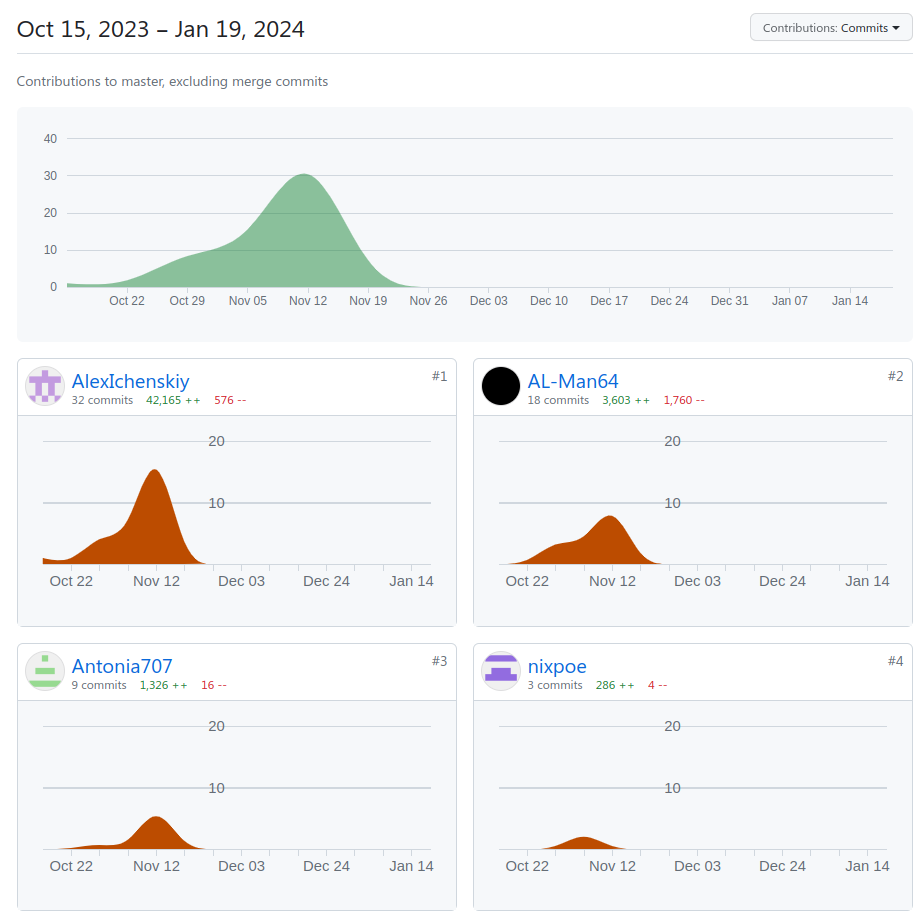
\includegraphics[scale=0.6]{slike/Contributors.png}
	\centering
	\caption{Prikaz aktivnosti na repozitoriju - 1. dio}
	\label{fig:repo_activiry_pt1}
\end{figure}

\begin{figure}[H]
	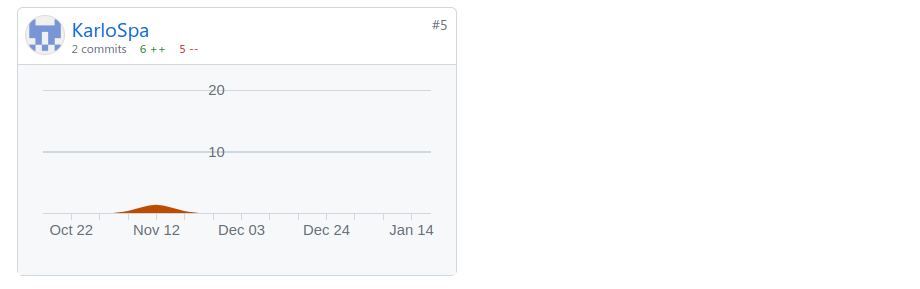
\includegraphics[scale=0.6]{slike/Contributors_Karlo.png}
	\centering
	\caption{Prikaz aktivnosti na repozitoriju - 2. dio}
	\label{fig:repo_activity_pt2}
\end{figure}

% TODO: ažurirati slike kad merge-amo sve u master
